\chapter{The Equivalence Principle and the Geometry of Gravity}

We begin where Einstein began: not with a finished geometric formalism, but with a very simple physical fact.  Gravity and acceleration look alike.  The lecture proceeds by making that statement precise in the most elementary Newtonian language, then by asking what sort of mathematics could possibly sustain it once we stop talking loosely and start talking in equations.  Only after the elevator thought experiment has been formalized do we turn to geometry, the metric tensor, and finally the tensor calculus that will be needed to decide whether the apparent ``curvy character'' of a metric is real or only an artifact of coordinates.

\section{Beginning with Einstein and the Equivalence Principle}

Susskind's chosen point of entry is methodological as much as physical.  General relativity is indeed a theory of geometry, but the lecture does not begin with geometry.  It begins with the equivalence principle, because Einstein's habit was to start from an elementary fact and then ask what consequences must follow if we take it seriously.

\begin{definition}
In the form that matters for the present lecture, the equivalence principle says that gravity and acceleration are locally indistinguishable: in a sufficiently small system, observed for a sufficiently short time, one cannot tell whether the observed force field is due to gravitation or to working in an accelerated frame of reference.
\end{definition}

A second methodological point is equally important.  At the outset we deliberately ignore special relativity.  We take
\[
t' = t
\]
and treat the speed of light as effectively infinite for slow motions.  This is not because special relativity is unimportant, but because the first job is to isolate the gravity--acceleration logic in its simplest form.  Once that logic is clear, the lecture will come back to Minkowski geometry and ask for the mathematics behind it.

\section{The Elevator Formalized in Newtonian Coordinates}

Consider an elevator moving vertically.  Let \(z\) be the vertical coordinate in a frame at rest with respect to the ground, and let \(z'\) be the vertical coordinate measured from the floor of the elevator.  If the floor of the elevator has height \(L(t)\) above the ground origin, then the relation between the two coordinate systems is
\begin{align}
z' &= z - L(t),\\
t' &= t,\\
x' &= x,
\end{align}
where we also assume that the elevator does not slide horizontally.

The lecture insists that it is worth writing this down explicitly, even though everybody already knows the physics, because this is our first example of a coordinate transformation and our first example of asking how laws of physics change under such a transformation.

\paragraph{Inertial case.}
If the elevator moves with uniform velocity \(v\), then
\begin{equation}
L(t)=vt,
\end{equation}
so that
\begin{equation}
z' = z - vt.
\end{equation}
Now take Newton's law in the vertical direction:
\begin{equation}
F = m \ddot z.
\end{equation}
Differentiating the transformation twice gives
\begin{equation}
\ddot z' = \ddot z,
\end{equation}
since the second derivative of \(vt\) vanishes.  Therefore the law of motion in the primed frame has exactly the same form:
\begin{equation}
F = m \ddot z'.
\end{equation}
This is of course just the Newtonian statement that all inertial frames are equivalent, but Susskind wants us to see it as a statement about coordinate transformations.

\begin{figure}[htbp]
\centering

\includegraphics[width=0.82\textwidth]{lecture_01_figure_02.png}
\caption{Newton's law specialized to the vertical coordinate.  The screenshot is worth keeping because it documents the moment when the familiar \(F=ma\) is narrowed to the one-dimensional vertical equation \(F=m\ddot z\).}
\end{figure}

\paragraph{Accelerated case.}
Now change only one ingredient.  Let the elevator accelerate uniformly upward with acceleration \(g\).  Then
\begin{equation}
L(t)=\frac{1}{2}gt^2,
\end{equation}
and the coordinate transformation becomes
\begin{equation}
z' = z - \frac{1}{2}gt^2.
\end{equation}
Differentiating,
\begin{align}
\dot L &= gt,\\
\ddot L &= g,
\end{align}
and therefore
\begin{equation}
\ddot z' = \ddot z - g.
\end{equation}
The transcript contains a visible sign check here, and one should preserve that rhythm in the prose: the point is not that the sign is mysterious, but that the lecture really does pause to make sure the Newtonian-looking force is placed on the correct side of the equation.  Rewriting the last equation as
\begin{equation}
\ddot z = \ddot z' + g,
\end{equation}
we substitute into Newton's law and obtain
\begin{equation}
F = m(\ddot z' + g).
\end{equation}
If we want the equation to look Newtonian in the primed frame, we move the extra term to the right-hand side:
\begin{equation}
m\ddot z' = F - mg.
\end{equation}

This is the first real payoff.  In the accelerated frame there appears an extra force term proportional to the mass.  That is exactly the special feature of gravity.  If the force itself is proportional to \(m\), then the mass cancels from the equation of motion, and the trajectory of a freely falling object does not depend on its mass.  That is why acceleration does not merely produce an inconvenient correction to Newton's law; it produces something with precisely the kinematic character of a uniform gravitational field.

\section{Curvilinear Coordinates, Space-Time Pictures, and the Bending of Light}

At this point the lecture pivots from algebra to geometry.  The transformation
\[
z' = z - vt
\]
is linear.  When we draw the coordinates in the \(z\)-\(t\) plane, straight lines go to straight lines.  That had better be so: a free particle moves in a straight line in space-time in one inertial frame, and it must still do so in another inertial frame.

\begin{figure}[htbp]
\centering
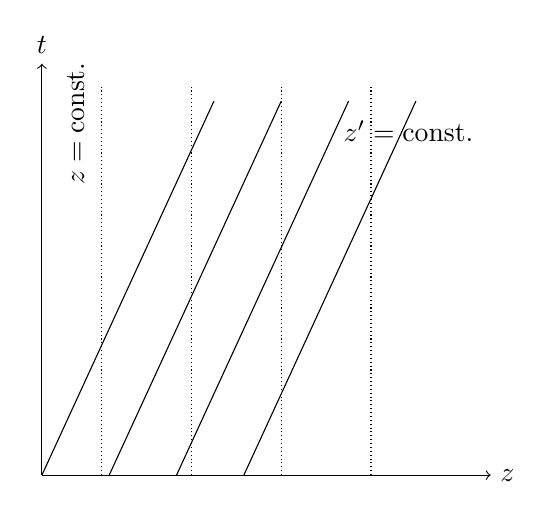
\begin{tikzpicture}[scale=0.95]
\draw[->] (0,0) -- (6,0) node[right] {$z$};
\draw[->] (0,0) -- (0,5.5) node[above] {$t$};
\foreach \a in {0.8,2.0,3.2,4.4} {
  \draw[densely dotted] (\a,0) -- (\a,5.2);
}
\foreach \b in {0.0,0.9,1.8,2.7} {
  \draw (\b,0) -- (\b+2.3,5.0);
}
\node at (4.9,4.6) {$z'=\mathrm{const.}$};
\node[rotate=90] at (0.45,4.7) {$z=\mathrm{const.}$};
\end{tikzpicture}
\caption{A schematic linear coordinate transformation in the \(z\)-\(t\) plane.  The \(z=\mathrm{const.}\) lines remain straight, and the \(z'=\mathrm{const.}\) lines are also straight.}
\end{figure}

The accelerated transformation,
\[
z' = z - \frac{1}{2}gt^2,
\]
is different.  Now the worldlines of fixed \(z'\) become parabolas lying on their side.  The lecture lingers on this because it is the beginning of the connection between gravity and curvilinear coordinate transformations of space-time.

\begin{figure}[htbp]
\centering
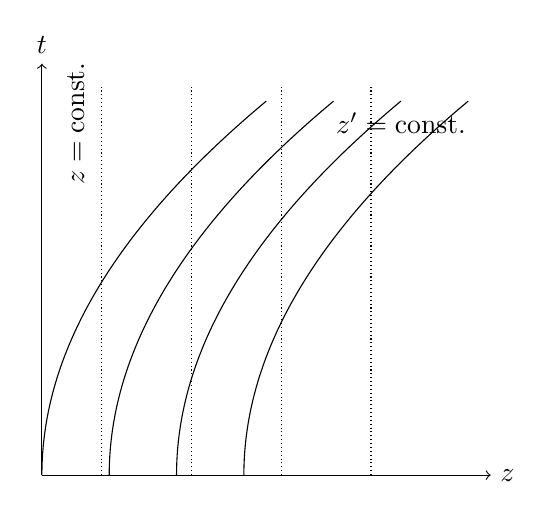
\begin{tikzpicture}[scale=0.95]
\draw[->] (0,0) -- (6,0) node[right] {$z$};
\draw[->] (0,0) -- (0,5.5) node[above] {$t$};
\foreach \a in {0.8,2.0,3.2,4.4} {
  \draw[densely dotted] (\a,0) -- (\a,5.2);
}
\foreach \b in {0.0,0.9,1.8,2.7} {
  \draw[smooth,domain=0:5,samples=60] plot ({0.12*\x*\x+\b},{\x});
}
\node at (4.8,4.7) {$z'=\mathrm{const.}$};
\node[rotate=90] at (0.45,4.7) {$z=\mathrm{const.}$};
\end{tikzpicture}
\caption{A schematic accelerated coordinate system.  The \(z=\mathrm{const.}\) lines remain straight, but the \(z'=\mathrm{const.}\) lines are parabolas, so straight lines in one frame need not be straight in the other.}
\end{figure}

Now comes Einstein's first nontrivial application of the principle.  Take a horizontal light ray emitted at \(t=0\).  In the unprimed frame, with no gravitational field present, it satisfies
\begin{equation}
x = ct,\qquad z=0.
\end{equation}
Using the accelerated-coordinate relation
\begin{equation}
z = z' + \frac{1}{2}gt^2,
\end{equation}
we find, after setting \(z=0\),
\begin{equation}
z' + \frac{1}{2}gt^2 = 0,\qquad x=ct.
\end{equation}
So the light ray is curved in the accelerated frame.  One may say that the elevator accelerates upward and the beam only appears to fall, but Einstein's point is exactly that the distinction is not physical at this local level.  If acceleration and gravity are equivalent in the required sense, then gravity must bend light.

\section{Real Gravity, Tidal Forces, and the Local Form of the Principle}

Up to now the discussion has been almost too successful.  It might sound as though any gravitational field can be created, or removed, by choosing funny coordinates.  Susskind deliberately stops here and raises the objection himself.

A real gravitational field, such as the radial field produced by the Earth or the Sun, points toward the center.  One can always choose a small freely falling laboratory in which gravity disappears locally, but no global coordinate transformation can remove the entire radial field everywhere at once.  If one point is made locally free, another point is generally made worse.

The physical reason is tidal force.  Take an extended object instead of a point particle.  The famous lecture example is the ``2,000 mile man.''  If he falls feet first toward a gravitating body, his feet feel a stronger pull than his head, and he is stretched.  If he falls sideways, the geometry of the radial field produces compression.  These are not coordinate artifacts.  They are invariant, physically detectable stresses on freely falling matter.

\subsection{Question \& Answer}

The lecture naturally poses the question this way: can gravity always be transformed away?

The answer is no.  What can be transformed away is a uniform, local gravitational field, the sort of field that appears in a sufficiently small freely falling laboratory.  What cannot be transformed away are tidal effects, because they measure variation of the field across an extended body.

That is why the careful statement of the equivalence principle is local.  If the system is small enough that the gravitational field does not vary appreciably from one part of it to another, then the distinction between gravity and acceleration disappears to that accuracy.  If the system is large enough for one part of it to be stretched while another is squeezed, then the distinction reappears.

The lecture then broadens the point.  It is not only uniformly accelerated elevators that produce fictitious gravitational fields.  Polar coordinates, rotating coordinates, or oscillating accelerated frames can generate centrifugal, Coriolis, and more complicated effective forces.  All of them can look gravitational.  But if there are no tidal distortions of a freely falling object, then the field is not genuine.

\section{From the Minkowski Interval to the Metric Tensor}

Once the local obstruction has been exposed, the lecture changes gears.  We ``take a rest from gravity'' and return to special relativity, because special relativity already teaches us that space-time carries geometry.

For neighboring events in one spatial and one temporal direction, Susskind recalls the invariant interval in the form
\begin{equation}
d\tau^2 = dt^2 - dx^2.
\end{equation}
Some authors prefer the opposite sign and write instead
\begin{equation}
ds^2 = dx^2 - dt^2.
\end{equation}
If one wishes to keep \(c\) explicit, one may write \(dx^2/c^2\) and then absorb the factor into a redefinition of the coordinate.  The essential point is not the sign convention, but the existence of a local geometric quantity that survives coordinate changes.

Now we step back from Minkowski space and ask the Euclidean question.  In ordinary flat space with Cartesian coordinates,
\begin{equation}
ds^2 = \sum_i (dx^i)^2 = \delta_{mn}\,dx^m dx^n.
\end{equation}
That is simply the Pythagorean theorem in any number of dimensions.  But on a curved surface, or even on a flat surface described by curvilinear coordinates, the distance between neighboring points takes a more general quadratic form:
\begin{equation}
ds^2 = \sum_{m,n} g_{mn}(x)\,dx^m dx^n.
\end{equation}
The coefficients \(g_{mn}(x)\) form the metric tensor.

The sphere provides the first concrete example.  In standard angular coordinates one may write
\begin{equation}
ds^2 = R^2\bigl(d\theta^2 + \sin^2\theta\,d\phi^2\bigr),
\end{equation}
if \(\theta\) is measured from the pole.  If instead \(\theta\) is measured from the equator, then the same geometry is described by
\begin{equation}
ds^2 = R^2\bigl(d\theta^2 + \cos^2\theta\,d\phi^2\bigr).
\end{equation}
The lecture is careful here: the coefficient of \(d\phi^2\) depends on convention, but the deeper lesson is independent of convention.  Distances are no longer given by a constant Euclidean matrix; they are governed by functions of position.

\begin{figure}[htbp]
\centering

\includegraphics[width=0.82\textwidth]{lecture_01_figure_03.png}
\caption{General line element over a local curved coordinate patch.  The board layout is important here: a local axis sketch, a small curvilinear-grid inset, and a larger coordinate patch all sit near the displayed formula for the metric.}
\end{figure}

\begin{figure}[htbp]
\centering
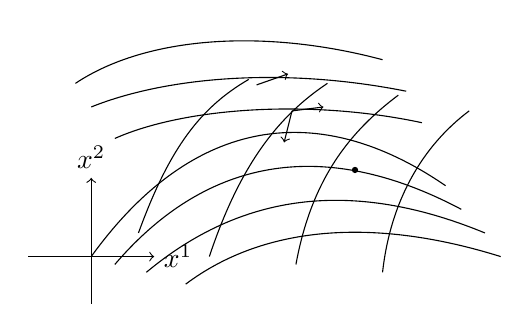
\begin{tikzpicture}[scale=1.0]
\draw[->] (-0.8,0) -- (0.8,0) node[right] {$x^1$};
\draw[->] (0,-0.6) -- (0,1.0) node[above] {$x^2$};

\draw[smooth] (-0.2,2.2) .. controls (0.7,2.8) and (2.2,2.9) .. (3.7,2.5);
\draw[smooth] (0.0,1.9) .. controls (1.0,2.3) and (2.5,2.4) .. (4.0,2.1);
\draw[smooth] (0.3,1.5) .. controls (1.2,1.9) and (2.8,2.0) .. (4.2,1.7);
\draw[->] (2.1,2.18) -- (2.5,2.32);

\draw[smooth] (0,0) .. controls (1.3,1.8) and (2.9,2.0) .. (4.5,0.9);
\draw[smooth] (0.3,-0.1) .. controls (1.5,1.3) and (3.0,1.5) .. (4.7,0.6);
\draw[smooth] (0.7,-0.2) .. controls (1.9,0.8) and (3.3,1.0) .. (5.0,0.3);
\draw[smooth] (1.2,-0.35) .. controls (2.2,0.4) and (3.6,0.5) .. (5.2,0.0);

\draw[smooth] (0.6,0.3) .. controls (1.0,1.4) and (1.4,1.9) .. (2.0,2.25);
\draw[smooth] (1.5,0.0) .. controls (1.9,1.2) and (2.4,1.8) .. (3.0,2.2);
\draw[smooth] (2.6,-0.1) .. controls (2.8,1.0) and (3.3,1.6) .. (3.9,2.05);
\draw[smooth] (3.7,-0.2) .. controls (3.8,0.7) and (4.2,1.4) .. (4.8,1.85);

\fill (3.35,1.1) circle (0.04);
\draw[->] (2.55,1.85) -- (2.95,1.90);
\draw[->] (2.55,1.85) -- (2.45,1.45);
\end{tikzpicture}
\caption{A schematic redraw of the local curved coordinate patch.  The metric is attached not to a global sphere picture, but to a local chart with two coordinate families, a marked point, and local differential directions.}
\end{figure}

\section{Intrinsic Geometry, Flatness, and One Metric Tensor}

At this stage the lecture asks us to be careful about what geometry means.  A folded page may look curved as an object embedded in three dimensions, but its intrinsic geometry may still be flat.  The distances measured along the page between neighboring points are the same whether the page is folded or unfolded.  That is the distinction between intrinsic and extrinsic geometry.

\begin{figure}[htbp]
\centering

\includegraphics[width=0.82\textwidth]{lecture_01_figure_04.png}
\caption{One metric tensor in a chosen coordinate chart.  This cleaner board state is useful because the line element and the local patch can both be read with less occlusion.}
\end{figure}

The lecture's central geometric question can now be stated sharply.  Suppose I hand you one metric tensor \(g_{mn}(x)\) in one coordinate system.  I have thereby told you the distance between every pair of neighboring points.  Can you tell whether the geometry is truly flat or only written in awkward coordinates?

\subsection{Question \& Answer}

Given one metric tensor, how do we test flatness?

The answer is not to look at one point.  At a point every smooth surface looks flat, and one may even diagonalize the metric there.  That does not settle the global question.  The real question is whether there exists a coordinate transformation that turns the metric into the Euclidean one everywhere:
\begin{equation}
g_{mn} \longrightarrow \delta_{mn}.
\end{equation}
If such a coordinate system exists globally, the space is flat.  If no such coordinate system exists, the space is curved.

This is why the lecture keeps insisting on the parallel with gravity.  Earlier the question was: can a gravitational field be removed by a coordinate transformation, or do tidal forces remain?  Now the question is: can the metric be turned into the Kronecker delta, or does its curvy character survive every coordinate change?

\begin{figure}[htbp]
\centering

\includegraphics[width=0.82\textwidth]{lecture_01_figure_05.png}
\caption{Pointing to the position-dependent metric factor.  The gesture matters because it fixes the spoken ``here'' to the coefficient \(g_{mn}(x)\), emphasizing that the metric depends on position.}
\end{figure}

The lecture returns once more to the local character of the construction.  The metric formula is a statement about neighboring points, not arbitrary separated points.  For finite separations one must know more of the geometry in between.  But the local quadratic form is enough to build the geometry piece by piece.

\begin{figure}[htbp]
\centering

\includegraphics[width=0.82\textwidth]{lecture_01_figure_06.png}
\caption{Folded surface sketch and local coordinate patch.  The left board is not a formal theorem diagram; it is evidence for the lecture's distinction between intrinsic distance relations and the way a surface may be folded in the surrounding space.}
\end{figure}

This is also the place where Susskind states the more exact relation between gravity and curvature.  The analogy is not merely suggestive.  In general relativity, tidal forces are diagnosed by curvature, and a flat space-time is one whose curvature tensor vanishes.  The lecture does not yet develop that machinery, but it tells us unambiguously where the story is heading.

\section{Tensor Analysis as the Next Tool}

To answer the flatness question we must know how geometric objects transform when we change coordinates.  This is why the lecture ends by opening tensor analysis.  It is not an ornament added to the physics.  It is the mathematics that the metric question has forced on us.

Susskind now changes notation.  Instead of \(x'^m\), he writes a second coordinate system as \(y^m\), simply to avoid miserable expressions with primes piled on indices.  Thus we have two coordinate systems \(x^m\) and \(y^m\), each understood as a smooth function of the other.

The differential coordinate change is the chain rule:
\begin{equation}
dy^m = \frac{\partial y^m}{\partial x^p}\,dx^p.
\end{equation}
Because the \(dx^m\) describe an infinitesimal vector from one point to a neighboring point, this equation becomes the model for a contravariant vector:
\begin{equation}
V'^m = \frac{\partial y^m}{\partial x^p}V^p.
\end{equation}
A contravariant vector is defined by transforming like this.

A different sort of object appears if we begin with a scalar function \(s(x)\).  Its gradient is
\begin{equation}
W_m = \frac{\partial s}{\partial x^m}.
\end{equation}
Applying the chain rule once more,
\begin{equation}
W'_m = \frac{\partial x^p}{\partial y^m}W_p.
\end{equation}
This is the defining transformation law for a covariant vector.  The lecture is careful to say that, at this stage, contravariant and covariant vectors are simply different kinds of objects.  Later the metric will relate them, but not yet.

The pattern for higher-rank tensors is built from products.  If \(V^m\) and \(U^n\) are contravariant vectors, then their product \(T^{mn}=V^mU^n\) transforms with one Jacobian for each upper index.  Likewise a tensor with two lower indices transforms with one inverse Jacobian for each lower index:
\begin{equation}
T'_{mn} = \frac{\partial x^p}{\partial y^m}\frac{\partial x^q}{\partial y^n}T_{pq}.
\end{equation}
The same pattern continues for more indices.

At this point Susskind explicitly introduces Einstein's summation convention.  Once an index is repeated in a term, we no longer write the summation sign.  The convenience is not merely typographical; it forces us to read formulas structurally, by their index pattern.

Finally, he returns to the metric:
\begin{equation}
ds^2 = g_{mn}(x)\,dx^m dx^n.
\end{equation}
If we rewrite the differentials in terms of the \(y\)-coordinates,
\begin{equation}
dx^m = \frac{\partial x^m}{\partial y^p}\,dy^p,
\end{equation}
then the interval can be rewritten in the new coordinates.  The lecture stops just before carrying this through completely, but the destination is clear: the metric transforms as a rank-2 covariant tensor.  Once we know that transformation law in detail, we may ask the hard mathematical question: can a given \(g_{mn}(x)\) be transformed into \(\delta_{mn}\), or not?

\section{Summary}

The lecture begins with the claim that gravity and acceleration are locally the same sort of thing, and it spends its first half making that claim concrete in Newtonian coordinates.  A uniformly accelerated elevator produces an apparent uniform gravitational field; a horizontal light ray becomes curved; and yet real gravitation cannot be reduced globally to a coordinate trick because tidal forces remain.

The second half then reframes the same issue geometrically.  The metric tensor tells us the distance between neighboring points.  Flatness means the existence of coordinates in which that metric becomes the Kronecker delta everywhere.  Curvature means that no such global coordinates exist.  To decide which is the case, we must know how vectors, gradients, and tensors transform.  That is the work postponed to the next lecture, where the metric's own transformation law and the relation between curvature and gravity will be taken up directly.